% !TEX root = ../document.tex
\section{Image Recognition mit TensorFlow}
\label{sec:Praxis}
In den nachfolgenden Kapitel soll mit TensorFlow ein Datenmodell retrainiert werden. Anschließend sollen beispielhaft einige Bilder klassifiziert werden. Um diese Punkte durchzuführen zu können, wird zunächst die Installation von TensorFlow auf einem Ubuntu 16.04 LTS installiert werden.

\subsection{Installation}
\label{subsec:inst}
Zunächst müssen alle Voraussetzungen für die Ausführung von TensorFlow vorbereitet werden. Hierfür muss Python\footnote{\url{https://www.python.org/}} 2.7 oder 3.x installiert werden. Unter Ubuntu kann ein Anwendung einfach über die Konsole aus der Packetverwaltung\footnote{\url{https://wiki.ubuntuusers.de/Paketverwaltung/}} installiert werden. Hierfür muss zunächst die Konsole mit der Tastenkombination \glqq{}STRG+ALT+T\grqq{} geöffnet werden und anschließend der entsprechende Befehl für Python 2.7 oder 3.x ausgeführt werden.

\begin{lstlisting}[frame=single]
sudo apt-get install python-pip python-dev   # Python 2.7
sudo apt-get install python3-pip python3-dev # Python 3.x
\end{lstlisting}

Anschließend kann TensorFlow über die Python-Paketverwaltung installiert werden. Hierfür muss einer der folgenden Befehle, je nachdem ob Python 2.7 oder 3.x verwendet werden soll, ausgeführt werden.

\begin{lstlisting}[frame=single]
pip install tensorflow      # Python 2.7
pip3 install tensorflow     # Python 3.x
\end{lstlisting}

Nachdem TensorFlow installiert ist, kann die Installation mithilfe einem kleinen Beispielprogramm getestet werden. Hierfür muss zunächst die interaktive Python-Eingabeaufforderung gestartet werden.

\begin{lstlisting}[frame=single]
python
\end{lstlisting}

Anschließend kann das nachfolgende Programm zur Überprüfung in die Eingabeaufforderungen eingegeben werden.

\begin{lstlisting}[frame=single]
import tensorflow as tf
hallo = tf.constant('Hallo, TensorFlow!')
session = tf.Session()
print(session.run(hallo))
\end{lstlisting}

Nachdem letzten Befehl sollte das Programm \glqq{}Hallo, TensorFlow!\grqq{} in der Eingabeaufforderung ausgeben.

\subsection{Image Retraining}
\label{subsec:trans-erstellung}
Im nachfolgenden Kapitel soll eine neue Bildklasse angelernt werden. Dafür wird mit dem vor trainierten Inception V3 Modell eine neue Bildkategorie antrainiert. Hierfür wird die beigefügte virtuelle Maschine verwendet. Das Passwort für den angelegten Benutzer der virtuellen Maschine lautet \glqq{}wert55wert\grqq{}. Innerhalb des Heimatverzeichnisse befinden sich die folgende Verzeichnis-Struktur.

\begin{figure}[!h]
	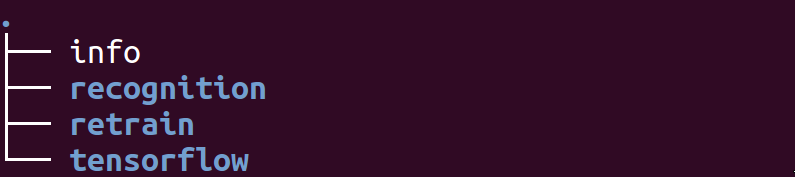
\includegraphics[width=\textwidth]{06.png}
	\caption{Verzeichnisstruktur Virtuelle Maschine}
	\label{fig:06}
\end{figure}

Alle benötigten Dateien befinden sich in dem \glqq{}retrain\grqq{}-Verzeichnis. In diesem Verzeichnis befindet sich einerseits das Python-Programm zum Retraining der neuen Klassen und ebenfalls die neu anzulernenden Klassen im \glqq{}images\grqq{}-Verzeichnis. Der Verzeichnisname beschreibt hierbei den Klassennamen und die darunterliegenden Dateien werden für das Retraining der Klasse verwendet.

\begin{figure}[!h]
	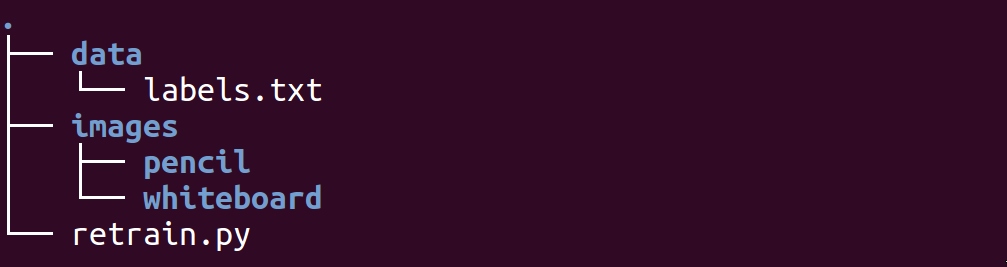
\includegraphics[width=\textwidth]{05.png}
	\caption{Verzeichnisstruktur \glqq{}retrain\grqq{}}
	\label{fig:05}
\end{figure}

\begin{figure}[!h]
	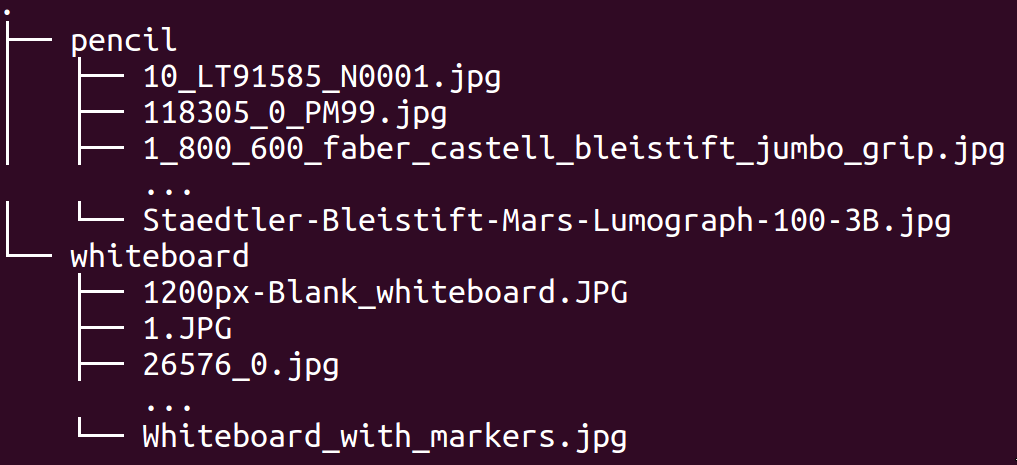
\includegraphics[width=\textwidth]{11.png}
	\caption{Verzeichnisstruktur der Klassen}
	\label{fig:11}
\end{figure}

Anschließend kann das Programm \glqq{}retrain.py\grqq{} mit dem folgenden Befehl ausgeführt werden.

\begin{lstlisting}[frame=single]
cd ~/tensorflow/retrain/
python retrain.py --image_dir=./images
\end{lstlisting}

Anschließend lädt das Programm das Inception V3 Modell herunter und führt das Retraining durch.

\begin{figure}[!h]
	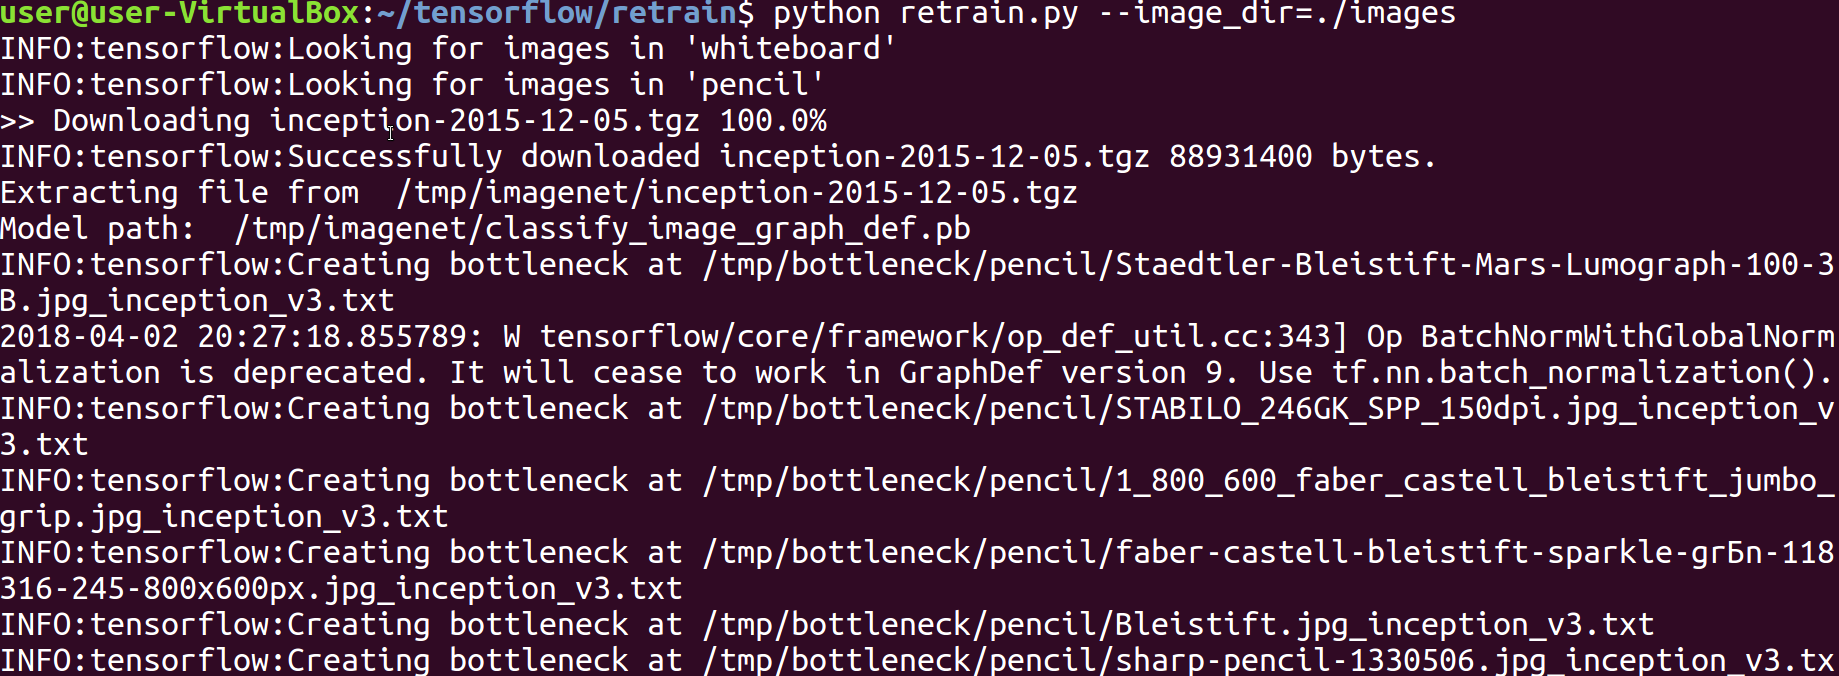
\includegraphics[width=\textwidth]{07.png}
	\caption{Retraining Konsolenausgaben: Bottleneck-Erstellung}
	\label{fig:07}
\end{figure}

Die Anwendung erstellt nun für jede vorhandene Datei eine sogenannte Bottleneckdatei. Hierbei handelt es sich um den vorfinalen Layer. Nachdem für jede Bilddatei eine Bottleneckdatei angelegt ist, wird das eigentliche Retraining durchgeführt. Die Ausgabe der Konsole sollte wie in Abbildung \ref{fig:08} dargestellt aussehen.

\begin{figure}[!h]
	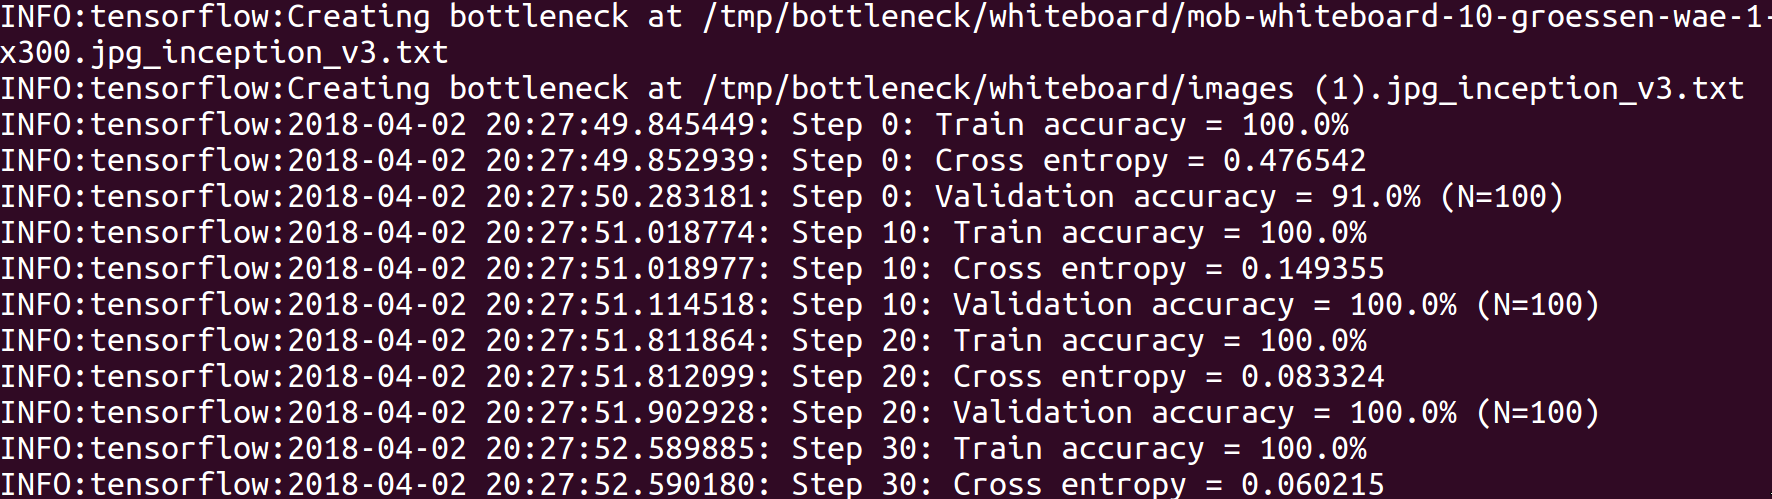
\includegraphics[width=\textwidth]{08.png}
	\caption{Retraining Konsolenausgaben: Retraining}
	\label{fig:08}
\end{figure}

Anschließend wird die Graph-Datei erstellt und die Bilderklassen wurden erfolgreich antrainiert.

\begin{figure}[!h]
	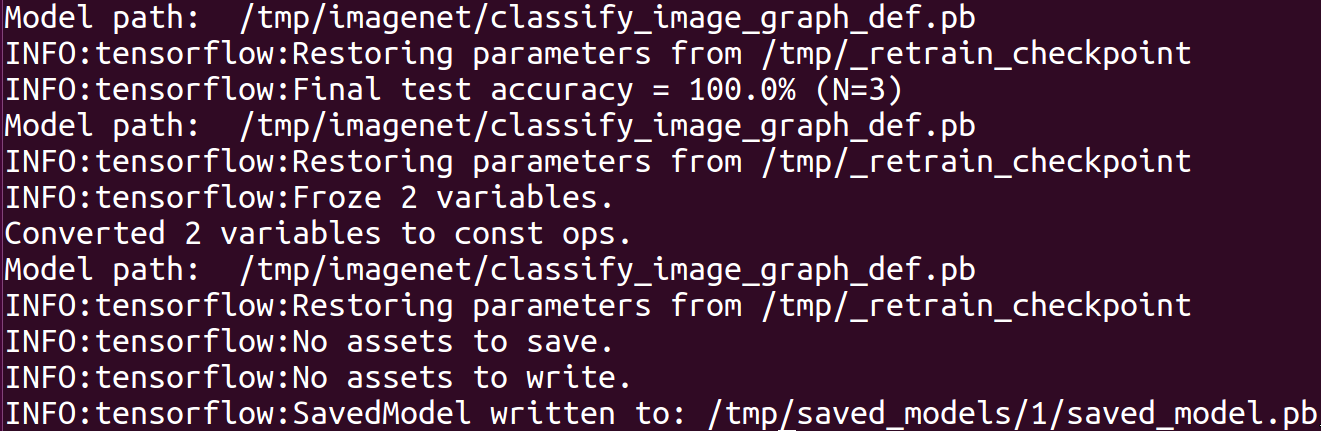
\includegraphics[width=\textwidth]{09.png}
	\caption{Retraining Konsolenausgaben: Graphdatei-Erstellung}
	\label{fig:09}
\end{figure}

\subsection{Image Recognition}
\label{subsec:trans-erstellung-mit-daten}
Nachdem die neuen Klassen antrainiert wurden, kann nun anschließend mit der Klassifizierung von Bildern begonnen werden. Hierfür werden die Dateien aus dem Verzeichnis \glqq{}recognition\grqq{} benötigt.

\begin{figure}[!h]
	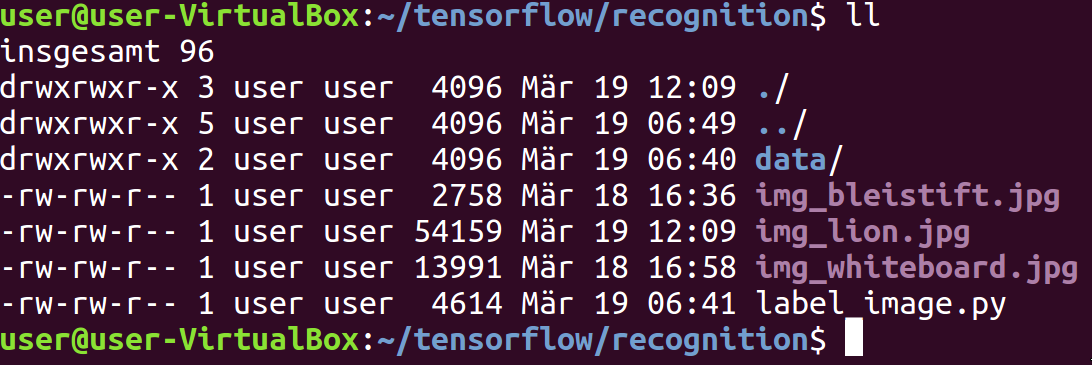
\includegraphics[width=\textwidth]{10.png}
	\caption{Recognition Verzeichnisstruktur}
	\label{fig:10}
\end{figure}

Um nun die neu trainierten Klassen zu verwenden müssen die Parameter bei Programmstart übergeben werden. Zunächst wird die vortrainierten Klassen getestet. Hierfür muss der folgende Befehl ausgeführt werden.

\begin{lstlisting}[frame=single]
cd ~/tensorflow/recognition/
python label_image.py --image=./img_whiteboard.jpg
\end{lstlisting}

Die Anwendung sollte das Bild des Whiteboards nicht erkennen, da die Whiteboard Klasse nicht in dem Inception V3 Modell vorhanden ist. Die Ausgabe sollte wie in Abbildung \ref{fig:12} dargestellt aussehen.

\begin{figure}[!h]
	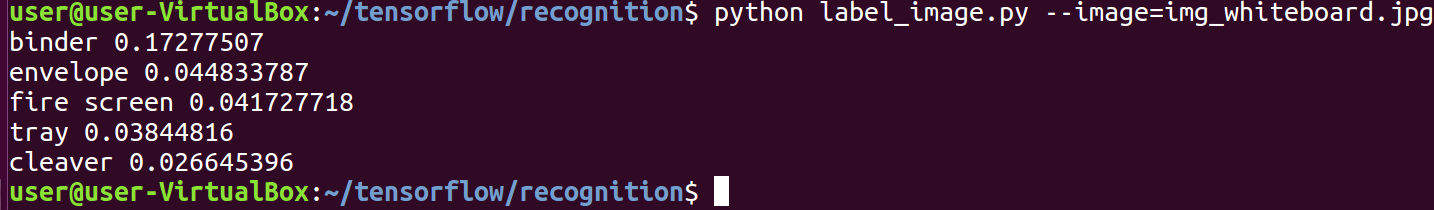
\includegraphics[width=\textwidth]{12.png}
	\caption{Recognition: Klasse nicht antrainiert}
	\label{fig:12}
\end{figure}

Anschließend wird mit dem folgenden Befehl ein Bild eines Löwen klassifiziert.

\begin{lstlisting}[frame=single]
cd ~/tensorflow/recognition/
python label_image.py --image=./img_lion.jpg
\end{lstlisting}

In diesem Beispiel sollte das neuronale Netz das Bild Klassifizieren können (Konsolenausgabe ist in Abbildung \ref{fig:13} dargestellt).

\begin{figure}[!h]
	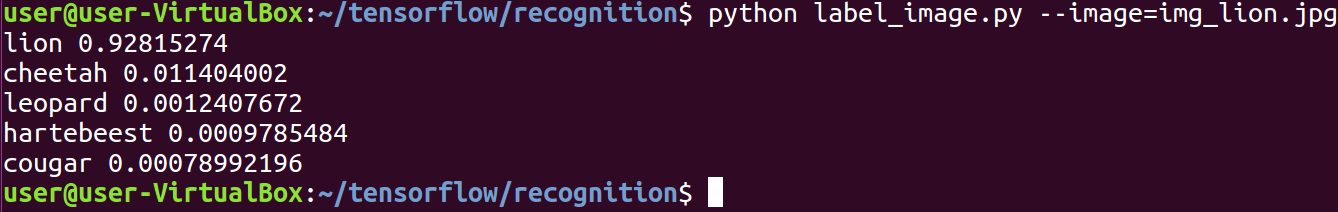
\includegraphics[width=\textwidth]{13.png}
	\caption{Recognition: Klasse antrainiert}
	\label{fig:13}
\end{figure}

Zuletzt wird das in Kapitel \ref{subsec:trans-erstellung} antrainierte Modell verwendet werden, sodass das Bild des Whiteboard erkannt werden kann. Hierfür müssen die Parameter der \glqq{}label\_image\grqq{}-Anwendung angepasst werden.

\begin{lstlisting}[frame=single]
cd ~/tensorflow/recognition/
python label_image.py --graph=/tmp/output_graph.pb --labels=output_labels --input_layer=Mul --output_layer=final_result --image=./img_whiteboard.jpg
\end{lstlisting}

Nachdem dieser Befehl ausgeführt ist, sollte die Konsole das Whiteboard klassifizieren können.

\begin{figure}[!h]
	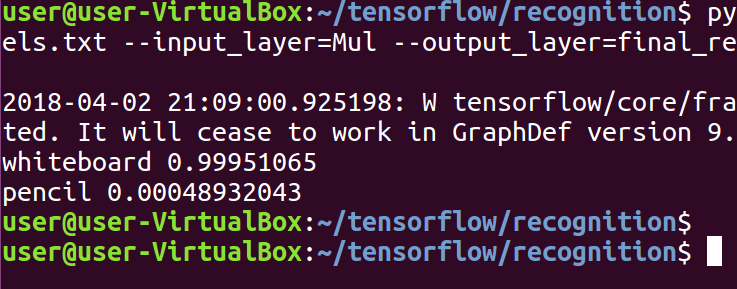
\includegraphics[width=\textwidth]{14.png}
	\caption{Recognition: Whiteboard erkannt}
	\label{fig:14}
\end{figure}

Der Parameter \glqq{}--graph\grqq{} steht für die Graph-Datei des trainierten neuronalen Netzwerks. Die Labels-Datei steht für die Klassen des Modells. Der Parameter \glqq{}--input\_layers\grqq{} definiert den Eingabe-Layer und \glqq{}--output\_layers\grqq{} den letzten Layer.
